%%%%%%%%%%%%%%%%%%%%%%%%%%%%%%%%%%%%%%%%%%%%%%%%%%%%%%%%%%%%%%%%%%%%%%%%%%%%%%%%%%%%%%%%%%%%%%%%%%%%%%%%%%%%%%%%%%%%%%%%%%%%%%%%%%%%%%%%%%%%%%%%%%%%%%%%%%%
% This is just an example/guide for you to refer to when submitting manuscripts to Frontiers, it is not mandatory to use Frontiers .cls files nor frontiers.tex  %
% This will only generate the Manuscript, the final article will be typeset by Frontiers after acceptance.   
%                                              %
%                                                                                                                                                         %
% When submitting your files, remember to upload this *tex file, the pdf generated with it, the *bib file (if bibliography is not within the *tex) and all the figures.
%%%%%%%%%%%%%%%%%%%%%%%%%%%%%%%%%%%%%%%%%%%%%%%%%%%%%%%%%%%%%%%%%%%%%%%%%%%%%%%%%%%%%%%%%%%%%%%%%%%%%%%%%%%%%%%%%%%%%%%%%%%%%%%%%%%%%%%%%%%%%%%%%%%%%%%%%%%

%%% Version 3.4 Generated 2022/06/14 %%%
%%% You will need to have the following packages installed: datetime, fmtcount, etoolbox, fcprefix, which are normally inlcuded in WinEdt. %%%
%%% In http://www.ctan.org/ you can find the packages and how to install them, if necessary. %%%
%%%  NB logo1.jpg is required in the path in order to correctly compile front page header %%%

\documentclass[utf8]{FrontiersinHarvard} % for articles in journals using the Harvard Referencing Style (Author-Date), for Frontiers Reference Styles by Journal: https://zendesk.frontiersin.org/hc/en-us/articles/360017860337-Frontiers-Reference-Styles-by-Journal
%\documentclass[utf8]{FrontiersinVancouver} % for articles in journals using the Vancouver Reference Style (Numbered), for Frontiers Reference Styles by Journal: https://zendesk.frontiersin.org/hc/en-us/articles/360017860337-Frontiers-Reference-Styles-by-Journal
%\documentclass[utf8]{frontiersinFPHY_FAMS} % Vancouver Reference Style (Numbered) for articles in the journals "Frontiers in Physics" and "Frontiers in Applied Mathematics and Statistics" 

%\setcitestyle{square} % for articles in the journals "Frontiers in Physics" and "Frontiers in Applied Mathematics and Statistics" 
\usepackage{url,hyperref,lineno,microtype,subcaption}
\usepackage[onehalfspacing]{setspace}

\linenumbers


% Leave a blank line between paragraphs instead of using \\


\def\keyFont{\fontsize{8}{11}\helveticabold }
\def\firstAuthorLast{Hernandez {et~al.}} %use et al only if is more than 1 author
\def\Authors{Christopher O. Hernandez\,$^{1}$, Joanne Labate\,$^{2}$, Bob Jarret\,$^{3}$, Kathleen Reitsma\,$^{4}$, Jack Fabrizio\,$^{5}$, Kan Bao\,$^{6}$, Zhangjun Fei\,$^{6,7}$, Rebecca Grumet\,$^{8}$ and Michael Mazourek$^{5*}$}
% Affiliations should be keyed to the author's name with superscript numbers and be listed as follows: Laboratory, Institute, Department, Organization, City, State abbreviation (USA, Canada, Australia), and Country (without detailed address information such as city zip codes or street names).
% If one of the authors has a change of address, list the new address below the correspondence details using a superscript symbol and use the same symbol to indicate the author in the author list.
\def\Address{$^{1}$ Department of Agriculture Nutrition and Food Systems, University of New Hampshire, Durham, NH, 03824 USA \\
$^{2}$Plant Genetic Resource Conservation Unit, United States Department of Agricultural Research Service, Geneva, NY, 14456 USA \\
$^{3}$Plant Genetic Resource Conservation Unit, United States Department of Agricultural Research Service, Griffin, GA, 30223 USA \\
$^{4}$North Central Regional Plant Introduction Station, Iowa State University, Ames, IA, 50014 USA \\
$^{5}$Plant Breeding and Genetics, Cornell University, Ithaca, NY, 14853 USA \\
$^{6}$Boyce Thompson Institute, Cornell University, Ithaca, NY, 14853 USA \\
$^{7}$U.S. Department of Agriculture-Agriculture Research Service, Robert W. Holley Center for Agriculture and Health, Ithaca, NY, 14853, USA \\
$^{8}$Department of Horticulture, Michigan State University, East Lansing, MI, 48824 USA }
% The Corresponding Author should be marked with an asterisk
% Provide the exact contact address (this time including street name and city zip code) and email of the corresponding author
\def\corrAuthor{Michael Mazourek}

\def\corrEmail{mm284@cornell.edu}




\begin{document}
\onecolumn
\firstpage{1}

\title {Characterization of the USDA \textit{Cucurbita pepo}, \textit{C. moschata}, and \textit{C. maxima Germplasm} Collections} 

\author[\firstAuthorLast ]{\Authors} %This field will be automatically populated
\address{} %This field will be automatically populated
\correspondance{} %This field will be automatically populated

\extraAuth{}% If there are more than 1 corresponding author, comment this line and uncomment the next one.
%\extraAuth{corresponding Author2 \\ Laboratory X2, Institute X2, Department X2, Organization X2, Street X2, City X2 , State XX2 (only USA, Canada and Australia), Zip Code2, X2 Country X2, email2@uni2.edu}


\maketitle


\begin{abstract}
The \emph{Cucurbita} genus is home to a number of economically and culturally important species.
We present the analysis of genotype data generated through genotyping-by-sequencing of the USDA germplasm collections of \emph{Cucurbita pepo}, \emph{C. moschata}, and \emph{C. maxima}.
These collections include a mixture of wild, landrace, and cultivated specimens from all over the world.
Roughly 1,500 - 32,000 high-quality single nucleotide polymorphisms (SNPs) were called in each of the collections, which ranged in size from 314 to 829 accessions.
Genomic analyses were conducted to characterize the diversity in each of the species and revealed extensive structure corresponding to a combination of geographical origin and morphotype/market class.
Genome-wide associate study (GWAS) was conducted for each data set using both historical and contemporary data, and signals were detected for several traits.
These data represent the largest collection of sequenced Cucurbita and can be used to direct the maintenance of genetic diversity and the development of breeding resources, and to help prioritize whole-genome re-sequencing for further GWAS and other genomics studies aimed at understanding the phenotypic and genetic diversity present in \emph{Cucurbita}.



\tiny
 \keyFont{ \section{Keywords:} Germplasm, Genotyping-by-sequencing, GWAS, Diversity, \textit{Cucurbita}} %All article types: you may provide up to 8 keywords; at least 5 are mandatory.
\end{abstract}

\section{Introduction}


The \emph{Cucurbitaceae} (Cucurbit) family is home to a number of vining species
mostly cultivated for their fruits.
This diverse and economically important family includes cucumber (\emph{Cucumis sativus}), melon (\emph{Cucumis melo}), watermelon (\emph{Citrullus lanatus}), and squash (\emph{Cucurbita ssp.})\citep{Ferriol}.
Like other cucurbits, squash exhibit diversity in growth habit, fruit morphology, metabolite content and disease resistance, and have a nuanced domestication story \citep{Chomicki2020,Paris2005}.
The genomes of \emph{Cucurbita ssp.} are small (roughly 400 Mb), but result from complex interactions between ancient genomes brought together through an allopolyploidization event \citep{Sun2017}.
These factors make squash an excellent model for understanding the biology of genomes, fruit development, and domestication.
Within \emph{Cucurbita}, five species are recognized as domesticated.
Three of these are broadly cultivated: \emph{C. maxima}, \emph{C. moschata}, and \emph{C. pepo} \citep{Ferriol}.
Few genomic resources have been available for these species; although, draft genomes and annotations, along with web-based tools and other genomics data are emerging \citep{Yu2022}.
Already, these resources have been used to elucidate the genetics of fruit quality, growth habit, disease resistance, and to increase the efficiency of cucurbit improvement \citep{MonteroPau2017,Zhong2017,Kazminska2018,Wu2019,Xanthopoulou2019,Hernandez2020}; however, there has yet to be a comprehensive survey of the genetic diversity in the large diverse \emph{Cucurbita} germplasm panels maintained by the USDA within the National Plant Germplasm System.

Germplasm collections play a vital role in maintaining and preserving genetic variation.
These collections can be mined by breeders for valuable alleles and can also be used by geneticists and biologists for mapping studies \citep{McCouch2020}.
Like many other orphan and specialty crops,there has been little effort put into developing community genetic resources for squash and other cucurbits.
The Cucurbit Coordinated Agricultural Project (CucCAP project) was established to help close the knowledge gap in cucurbits.
This collaborative project aims to provide genomics resources and tools that can aid in both applied breeding and basic research.
The genetic and phenotypic diversity present in the USDA watermelon, melon, and cucumber collections has already been explored as part of the CucCap project, partially through the sequencing of USDA germplasm collections and development of core collections for whole-genome sequencing \citep{Wang2021,Wang2018,Wu2019a}.
The diverse specimens of the USDA squash collections have yet to be well characterized at the genetic level;although, an elaborate system has been established for classifying squash based on species and various other characteristics.

The classification system used in squash is complex.
Squash from each species can be classed as winter or summer squash depending on whether the fruit is consumed at an immature or mature stage, the latter is a winter squash \citep{Loy2004}.
Squash are considered ornamental if they are used for decoration, and some irregularly shaped, inedible ornamental squash are called gourds; however, gourds include members of \emph{Cucurbita} as well as some species from \emph{Lagenaria}---not all gourds are squash \citep{Paris2015}.
Many squash are known as pumpkins; the pumpkin designation is a culture dependent colloquialism that can refer to jack O' lantern types, squash used for desserts or, in some Latin American countries, to eating squash from \emph{C. moschata} known locally as Calabaza \citep{Ferriol}.
Cultivars deemed as pumpkins can be found in all widely cultivated squash species.
Unlike the previous groupings, morphotypes/market classes are defined within species.
For example, a Zucchini is reliably a member of \emph{C. pepo} and a Buttercups are from \emph{C. maxima}.
Adding to the complexity of their classification, the \emph{Cucurbita} species are believed to have arisen from independent domestication events and the relationships between cultivated and wild species remains poorly understood \citep{Kates2017}.

\emph{C. pepo} is the most economically important of the \emph{Cucurbita} species and is split into two different subspecies: \emph{C. pepo} subsp. \emph{pepo} and \emph{C. pepo} subsp. \emph{ovifera} \citep{Xanthopoulou2019}.
Evidence points to Mexico as the center of origin for \emph{pepo} and southwest/central United States as the origin of \emph{ovifera}. The progenitor of \emph{ovifera} is considered by some to be subsp. \emph{ovifera} var. \emph{texana}, whereas subsp. \emph{fraterna} is a candidate progenitor for \emph{pepo} \citep{Kates2017}.
Europe played a crucial role as a secondary center of diversification for subsp. \emph{pepo}, but not subsp. \citep{Lust2016}.
Important morphoptypes of \emph{pepo} include Zucchini, Spaghetti squash, Cocozelle, Vegetable Marrow, and some ornamental pumpkins.
\emph{C. pepo} subsp. \emph{ovifera} includes summer squash from the Crookneck, Scallop, and Straightneck group, and winter squash such as Delicata and Acorn \citep{Paris2012}.

The origin of \emph{C. moschata} is more uncertain than \emph{C. pepo}; it is unclear whether \emph{C. moschata} has a South or North American origin \citep{Chomicki2020}.
Where and when domestication occurred for this species is also unknown; however, it is known that \emph{C. moschata} had an India-Myanmar secondary center of origin where the species was further diversified \citep{Sun2017}.
\emph{C. moschata} plays an important role in squash breeding as it is cross-fertile to various degrees with \emph{C. pepo} and \emph{C. maxima}, and can thus be used as a bridge to move genes across species \citep{Sun2017}.
Popular market classes of \emph{C. moschata} include cheese types like dickenson, which is widely used for canned pumpkin products, Butternut (Neck) types, Japonica, and tropical pumpkins known as Calabaza \citep{Ferriol}.

\emph{C. maxima} contains many popular winter squash including Buttercup/Kabocha types, Kuri, Hubbard, and Banana squash \citep{Ferriol}.
This species also sports the world's largest fruit, the giant pumpkin whose fruit are grown for competition and can reach well over 1000 Kg \citep{Savage015}.
Although this species exhibits a wide range of phenotypic diversity in terms of fruit characteristics, it appears to be the least genetically diverse of the three species described \citep{Kates2017}.
\emph{C. maxima} is believed to have a South American origin, and was likely domesticated near Peru, with a secondary center of domestication in Japan and China \citep{Nee1990,Sun2017}.

In this study, we set out to characterize the genetic diversity present in the USDA \emph{Cucurbita} germplasm collections for \emph{C. pepo}, \emph{C. moschata}, and \emph{C. maxima}.
We present genotyping-by-sequencing (GBS) data from each of these collections, population genomics analysis, results from genome-wide association study (GWAS) using historical and contemporary phenotypes, and suggest a core panel for re-sequencing.


\section{Materials and Methods}

\subsection{Plant Materials and Genotyping}
All available germplasm were requested from USDA cooperators for C. maxima (534 accessions from Geneva, NY), C. moschata (314 accessions from Griffin, GA), and C. pepo (829 accessions from Ames, IA) respectively. Seeds were planted in 50-cell trays and two 3/4 inch punches of tissue (approximately 80-150 mg) was sampled from the first true leaf of each seedling. DNA was extracted using Omega Mag-Bind Plant DNA DS kits (M1130, Omega Bio-Tek, Norcross, GA) and quantified using Quant-iT PicoGreen dsDNA Kit (Invitrogen, Carlsbad, CA). Purified DNA was shipped to Cornell’s Genomic Diversity Facility for GBS library preparation using protocols optimized for each species. Libraries were sequenced at either 96, 192, or 384-plex on the HiSeq 2500 (Illumina Inc., USA) with single-end mode and a read length of 101 bp.

\subsection{Variant Calling and Filtering}
SNP calling was conducted using the TASSEL-GBS V5 pipeline \citep{Glaubitz2014}. Tags produced by this pipeline were aligned using the default settings of the BWA aligner \citep{Li2009}. Raw variants were filtered using BCFtools \citep{Danecek2021}. Settings for filtering SNPs were as follows, minor allele frequency (MAF) $\geq 0.05$, missingness $\leq 0.4$, and biallelic. Three outlier genotypes were found in an initial principal components analysis (PCA) of the C. maxima data and were removed, as they were likely not C. maxima. Variants were further filtered for specific uses as described below.

\subsection{Population Genomics Analysis}
ADMIXTURE \citep{Alexander2011}, which uses a model-based approach to infer ancestral populations ($k$) and admixture proportions in a given sample, was used to explore population structure in each dataset. ADMIXTURE does not model linkage disequilibrium (LD); thus, marker sets were further filtered to obtain SNPs in approximate linkage equilibrium using the “–indep-pairwise” option in PLINK \citep{Purcell2007} with $r^{2}$ set to 0.1, a window size of 50 SNPs, and a 10 SNP step size . All samples labeled as cultivars or breeding material were removed from the data prior to running ADMIXTURE. Cross-validation was used to determine the best  value for each species. Briefly, ADMIXTURE was run with different  values (1-20) and the cross-validation error was reported for each $k$. The $k$ value with minimal cross-validation error was chosen for each species (Supplemental Figures, Figure 2). Ancestral populations were then assigned to cultivars using the program’s projection feature.

Principal components analysis (PCA) was used as a model-free way of determining population structure. PCA was conducted using SNPRelate \citep{} on the same LD-pruned data used by ADMIXTURE.

Linkage disequilibrium was calculated in each germplasm panel, and within each subgroup identified by ADMIXTURE.

Fst vales between.  

\subsection{Analysis of Phenotypic Data}
Historical data were obtained from the USDA Germplasm Resources Information Network (GRIN; www.ars-grin.gov) for C. maxima, C. pepo, and C. moschata. All duplicated entries were removed for qualitative traits, where categories are mutually exclusive, leaving only samples with unique entries for analysis. Two traits: adult and nymph squash bug damage in C. pepo where transformed using the boxcox procedure. Contemporary phenotypic data were collected from a subset of the C. pepo collection grown in the summer of 2018 in Ithaca, NY. Field-grown plants were phenotyped for vining bush habit at three different stages during the growing seasons to confirm bush, semi-bush or vining growth habit. Plants that had a bush habit early in the season but started to vine at the end of the season were considered semi-bush.

\subsection{GWAS}
Variant data were filtered to MAF  and missingness , and then imputed prior to association analysis. LinkImpute \citep{Money2015}, as implemented by the TASSEL \citep{Bradbury2007} “LDKNNiImputatioHetV2Plugin” plugin was used for imputation with default settings. Any data still missing after this process were mean imputed. The GENESIS \citep{} R package, which can model both binary and continuous traits. All models included the first two PCs of the marker matrix as fixed effects and modeled genotype effect () as a random effect distributed according to the kinship () matrix (). Binary traits were modeled using a logistic regression with GENESIS. The kinship matrix was calculated using A.mat from rrBLUP \citep{Endelman2011} with mean imputation.

\subsection{Genomic Heritability}

An estimate of genomic heritability \citep{Campos2015} was calculated for all ordinal and quantitative traits using a similar model an equivalent model to what was used for GWAS. Variance components from the random genetic effect and error were then used to calculate the heritability as .

\subsection{Syntenty of Bu putative region in C. pepo and C. maxima}
All tools used in the analysis can be found on the Cucurbit Genomics website (http://cucurbitgenomics.org/). A candidate gene for dwarfism, Bu, in C. maxima was elucidated by a previous study23 and was named Cma\_004516. The Cucurbit Genomics Database gene ID of Cma\_004516 was identified by using the BLAST tool to align primer sequences used for RT-QPCR in the previous study against the C. maxima reference genome. The synteny analysis was done by using the Synteny Viewer tool and evaluating C. maxima’s chromosome 3 with C. pepo’s chromosome 10 and searching for an ortholog to the candidate gene. The physical position of the C. pepo ortholog was identified by searching the gene using the Search tool. All tools used in the analysis can be found on the Cucurbit Genomics Database at cucurbitgenomics.org.

\subsection{Identification of a Core Collection}
Subsets representative of each panel’s genetic diversity were identified through running GenoCore \citep{Jeong2017} using the filtered SNP sets. The GenoCore settings were “-cv 99 -d 0.001”.


\section{Results}

\section{Discussion}


\section*{Conflict of Interest Statement}
Michael Mazourek is a co-founder of Row 7 Seeds, but neither receives compensation nor holds equity.

\section*{Author Contributions}



\section*{Funding}

Funding was provided by \textbf{Insert grant identifier here} as part of the Cucurbit Coordinate Agriculture Project.

\section*{Acknowledgments}
This work was supported by CucCAP, a USDA-NIFA-SCRI competitive grant 2015-51181-24285. We thank Kyle LaPlant for plant phenotyping assistance, and Sue Hammer and Paige Reeves for assistance with DNA extraction.

\section*{Data Availability Statement}
The datasets generated for this study includeing variant and raw sequence data are available on the Cucurbit Genomics Dataase at \href{https://cucurbitgenomics.org}{cucurbitgenomics.org}. The phenotypic data used are available for download from the USDA Germplasm Resources Information Network (GRIN; \href{https://www.ars-grin.gov}{www.ars-grin.gov}). Intermediate files and code used in the study are available on Github at \href{https://www.github.com/ch728/Cucurbita-USDA}{www.github.com/ch728/Cucurbita-USDA}.

\bibliographystyle{Frontiers-Harvard} %  Many Frontiers journals use the Harvard referencing system (Author-date), to find the style and resources for the journal you are submitting to: https://zendesk.frontiersin.org/hc/en-us/articles/360017860337-Frontiers-Reference-Styles-by-Journal. For Humanities and Social Sciences articles please include page numbers in the in-text citations 
%\bibliographystyle{Frontiers-Vancouver} % Many Frontiers journals use the numbered referencing system, to find the style and resources for the journal you are submitting to: https://zendesk.frontiersin.org/hc/en-us/articles/360017860337-Frontiers-Reference-Styles-by-Journal
\bibliography{cuccap-fresh}

%%% Make sure to upload the bib file along with the tex file and PDF
%%% Please see the test.bib file for some examples of references

\section*{Figure captions}

%%% Please be aware that for original research articles we only permit a combined number of 15 figures and tables, one figure with multiple subfigures will count as only one figure.
%%% Use this if adding the figures directly in the mansucript, if so, please remember to also upload the files when submitting your article
%%% There is no need for adding the file termination, as long as you indicate where the file is saved. In the examples below the files (logo1.eps and logos.eps) are in the Frontiers LaTeX folder
%%% If using *.tif files convert them to .jpg or .png
%%%  NB logo1.eps is required in the path in order to correctly compile front page header %%%

\begin{figure}[h]
\begin{center}
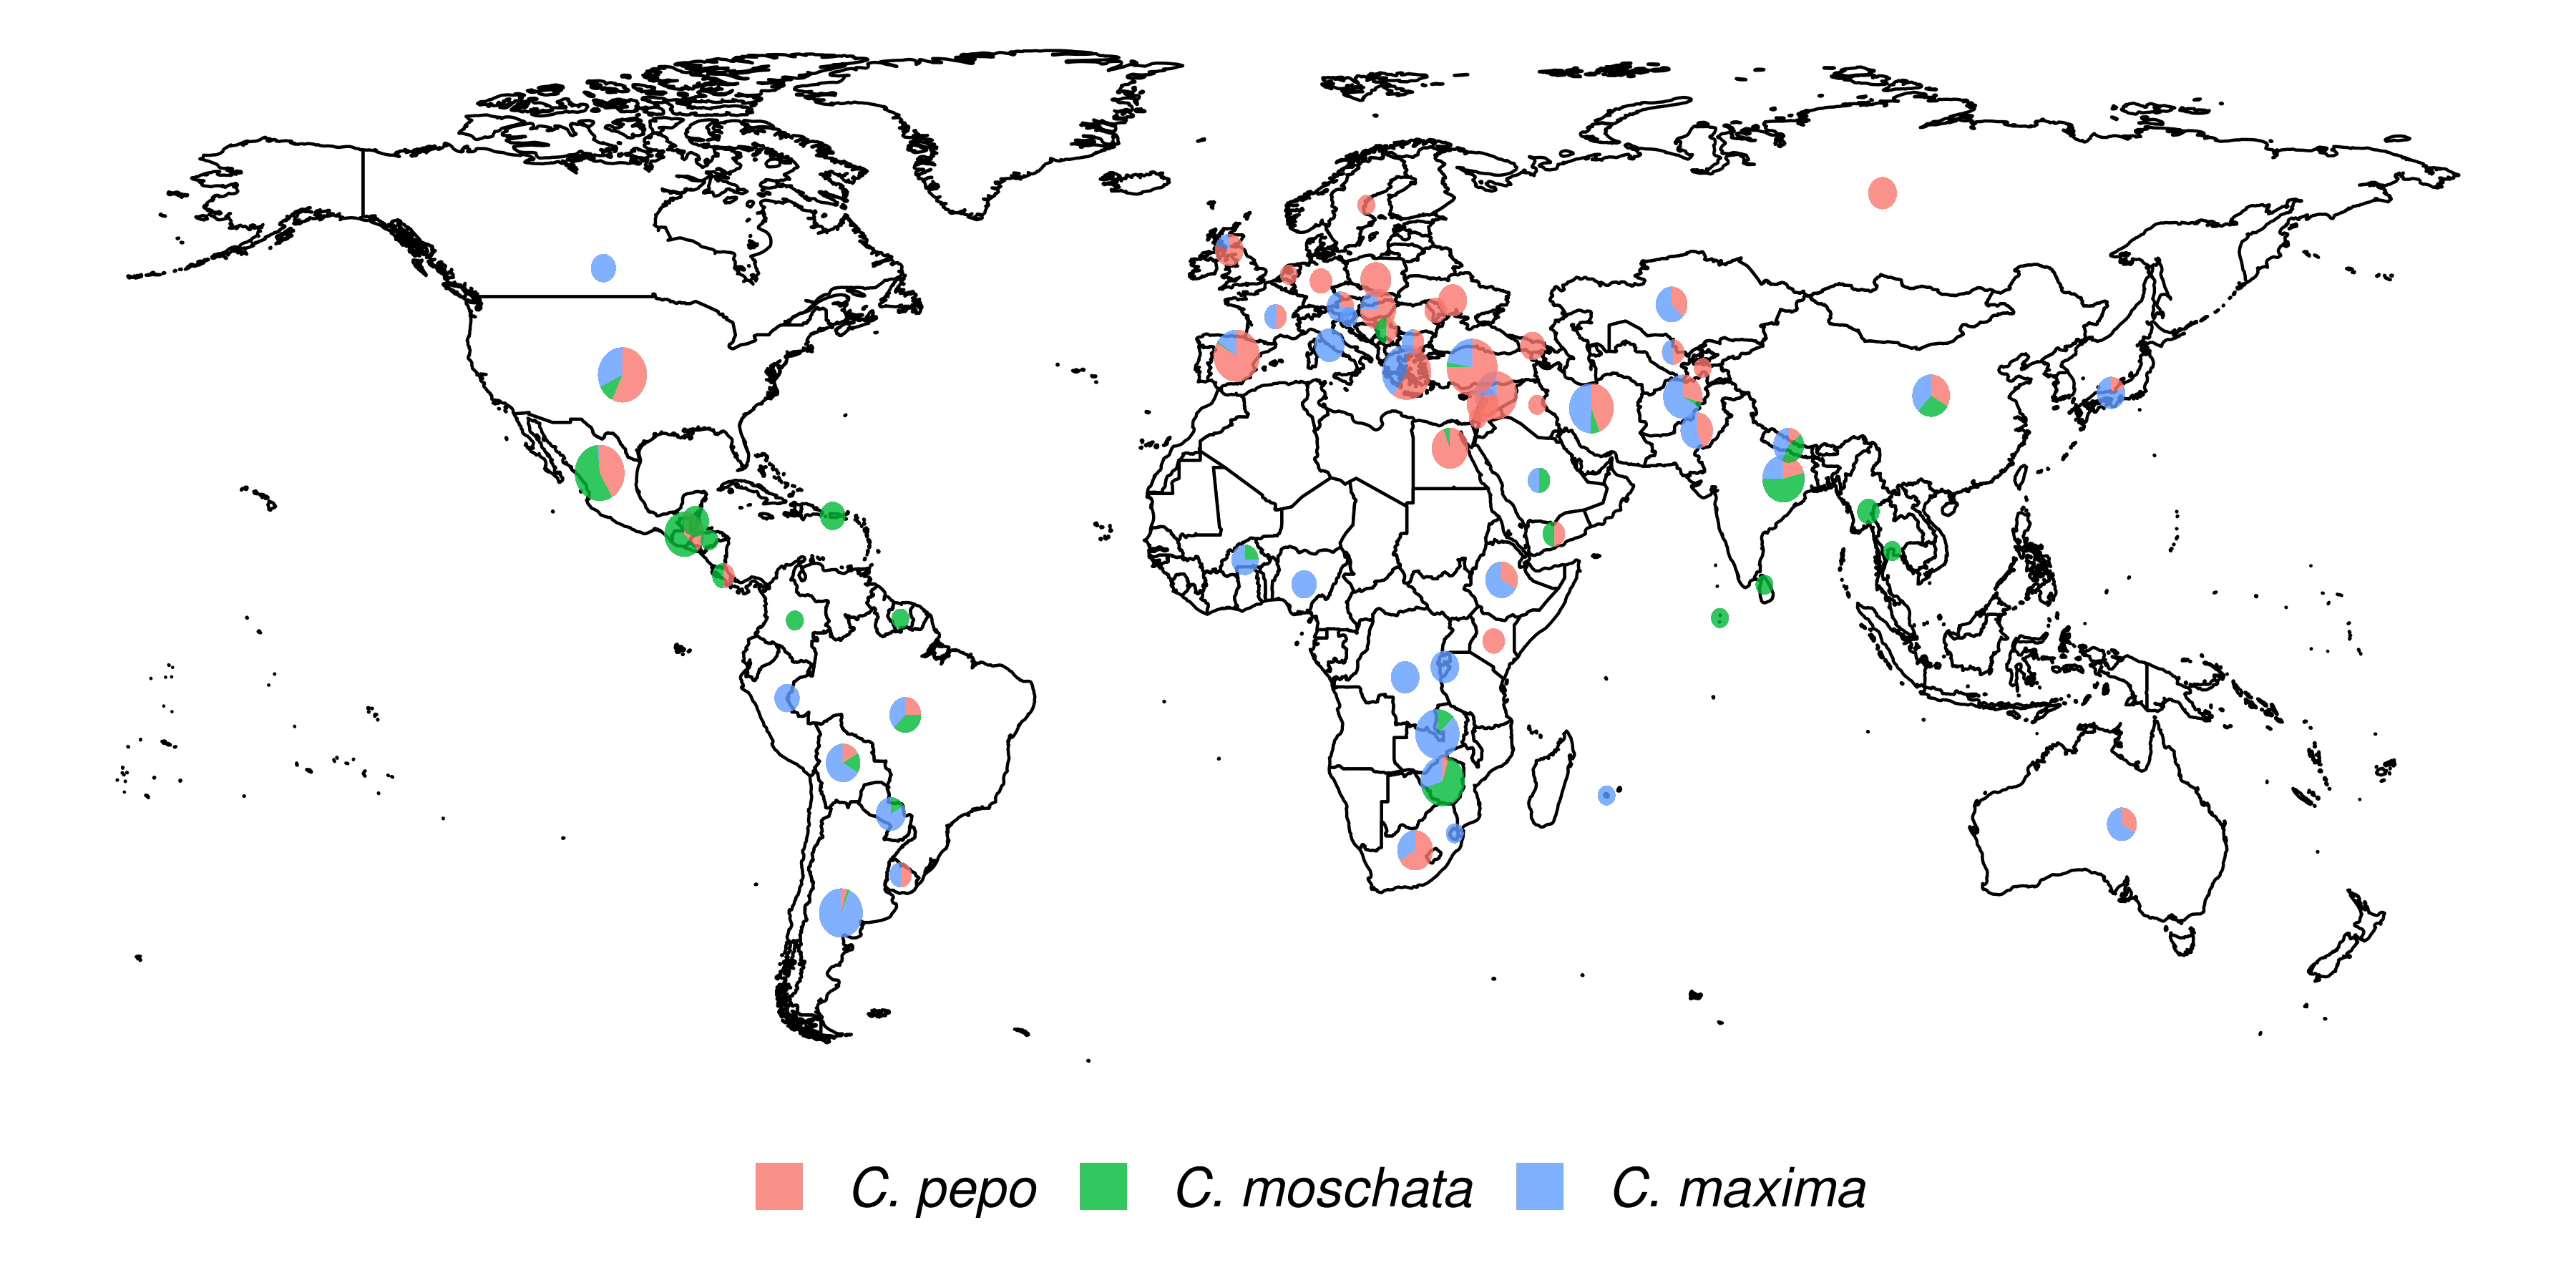
\includegraphics[width=15cm]{../../figures/01_fig.png}% This is a *.eps file
\end{center}
\caption{Geographical distribution of the USDA Cucurbita ssp. collection. The size of the pie chart is scaled according to the number of accessions and sector areas correspond to the proportion of the three species. \label{fig:1}}
\end{figure}

\begin{figure}[h]
	\begin{center}
		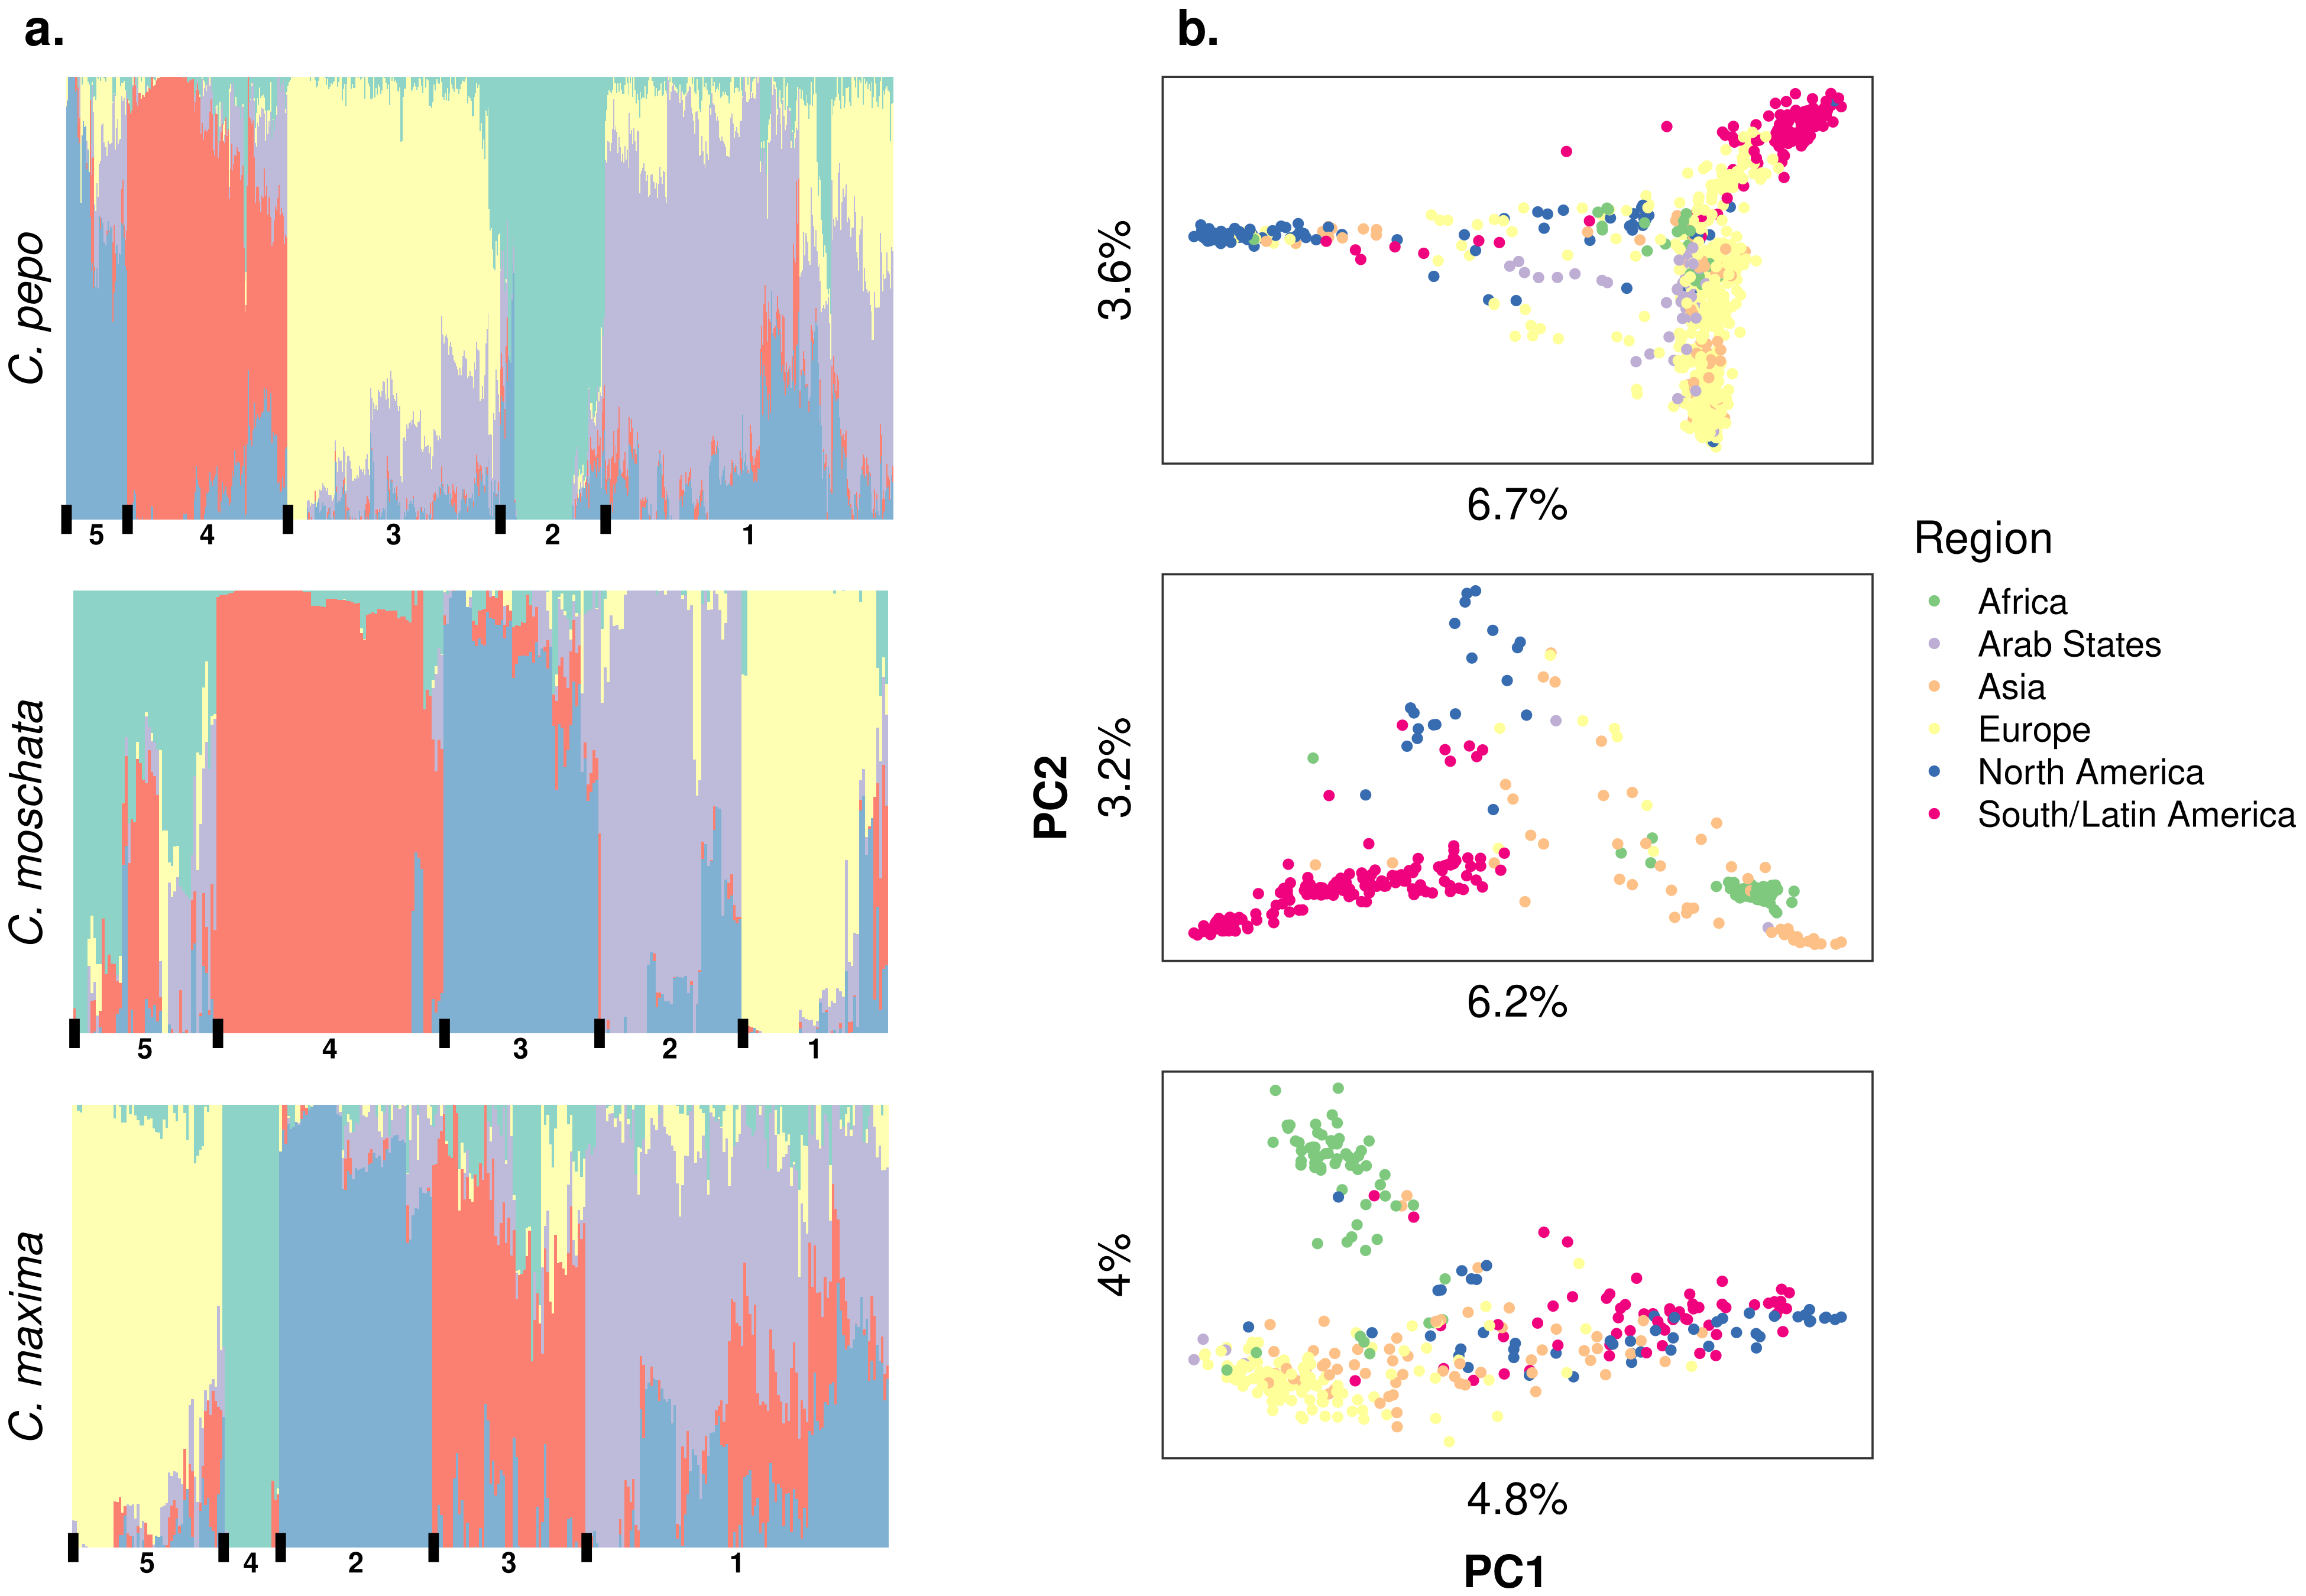
\includegraphics[width=18cm]{../../figures/02_fig.png}% This is a *.eps file
	\end{center}
	\caption{Population structure results aligned vertically by species. Panel a. Admixture plots: each stacked barplot represents an accession colored by proportion of inferred ancestral population. Groups based on hierarchical clustering are delimited by vertical bars and labeled with numbers along the bottom. Panel b. Plots of the first two principal components (PC) of accessions colored by region, variation explained by PCs is labeled on each axis. \label{fig:2}}
\end{figure}

\begin{figure}[h]
	\begin{center}
		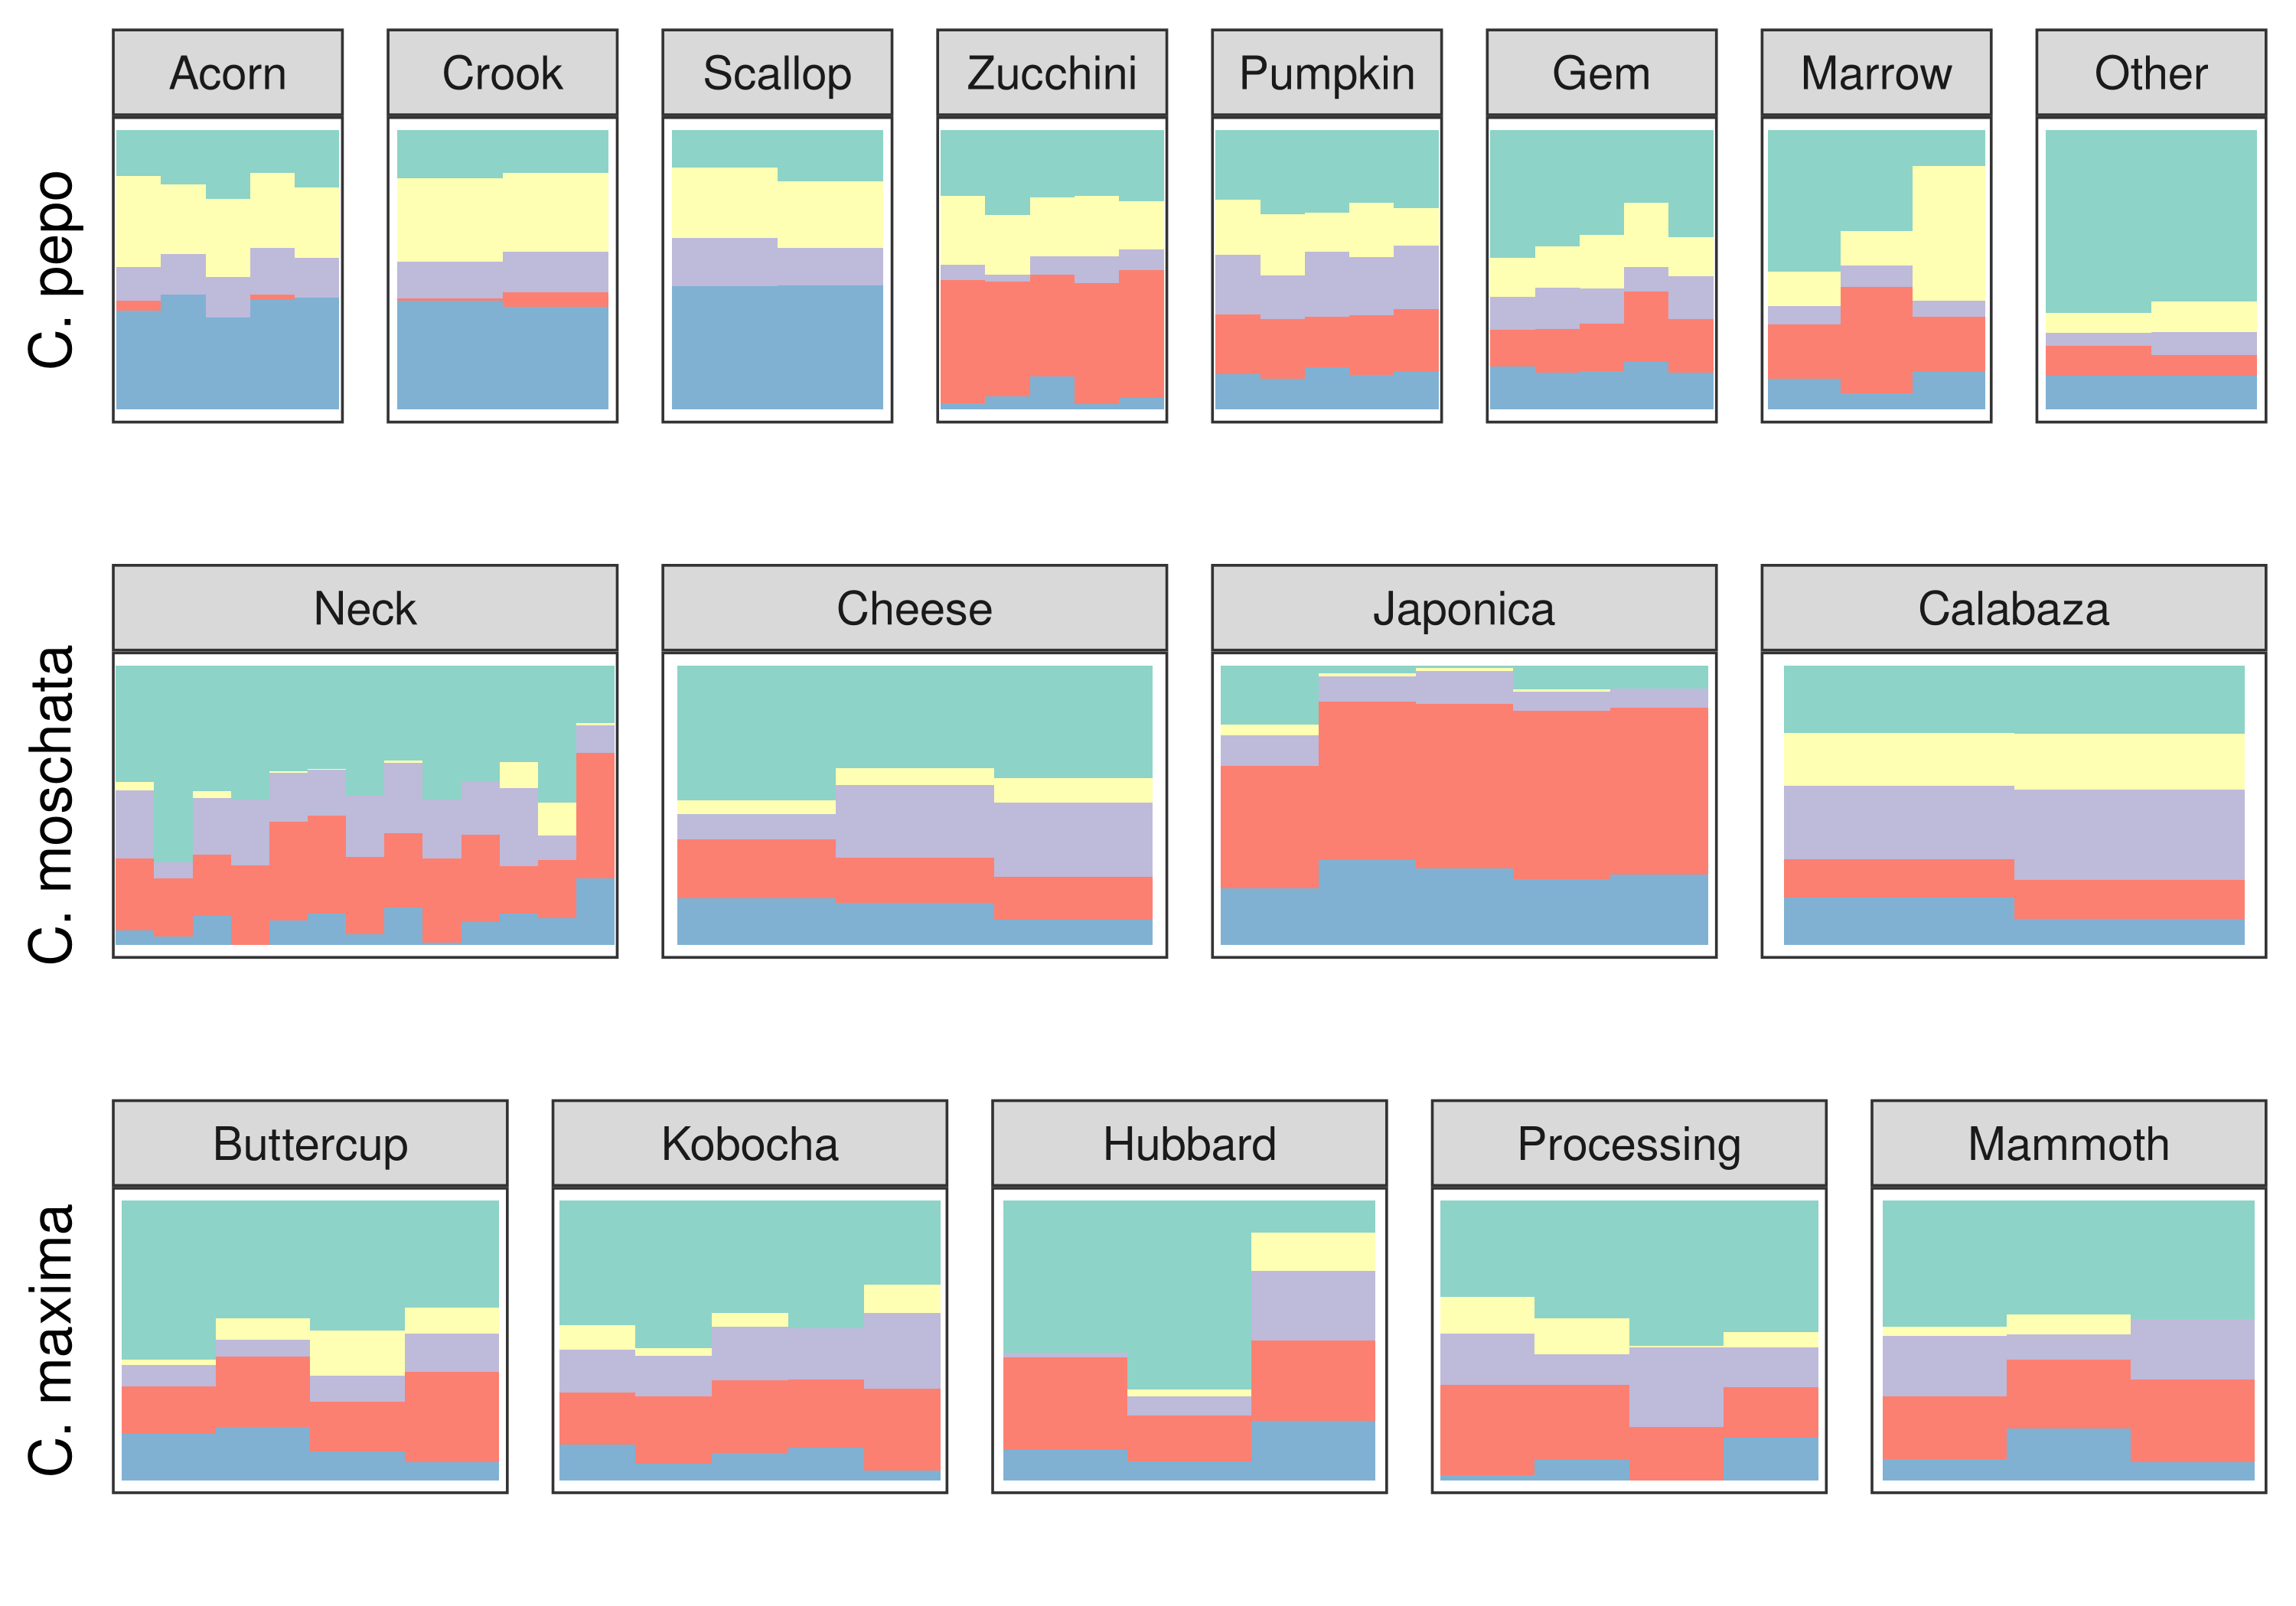
\includegraphics[width=15cm]{../../figures/03_fig.png}% This is a *.eps file
	\end{center}
	\caption{Ancestry coefficients projected on cultivars from each species. Results are shown grouped by market/varietal class. \label{fig:3}}
\end{figure}


\begin{figure}[h]
	\begin{center}
		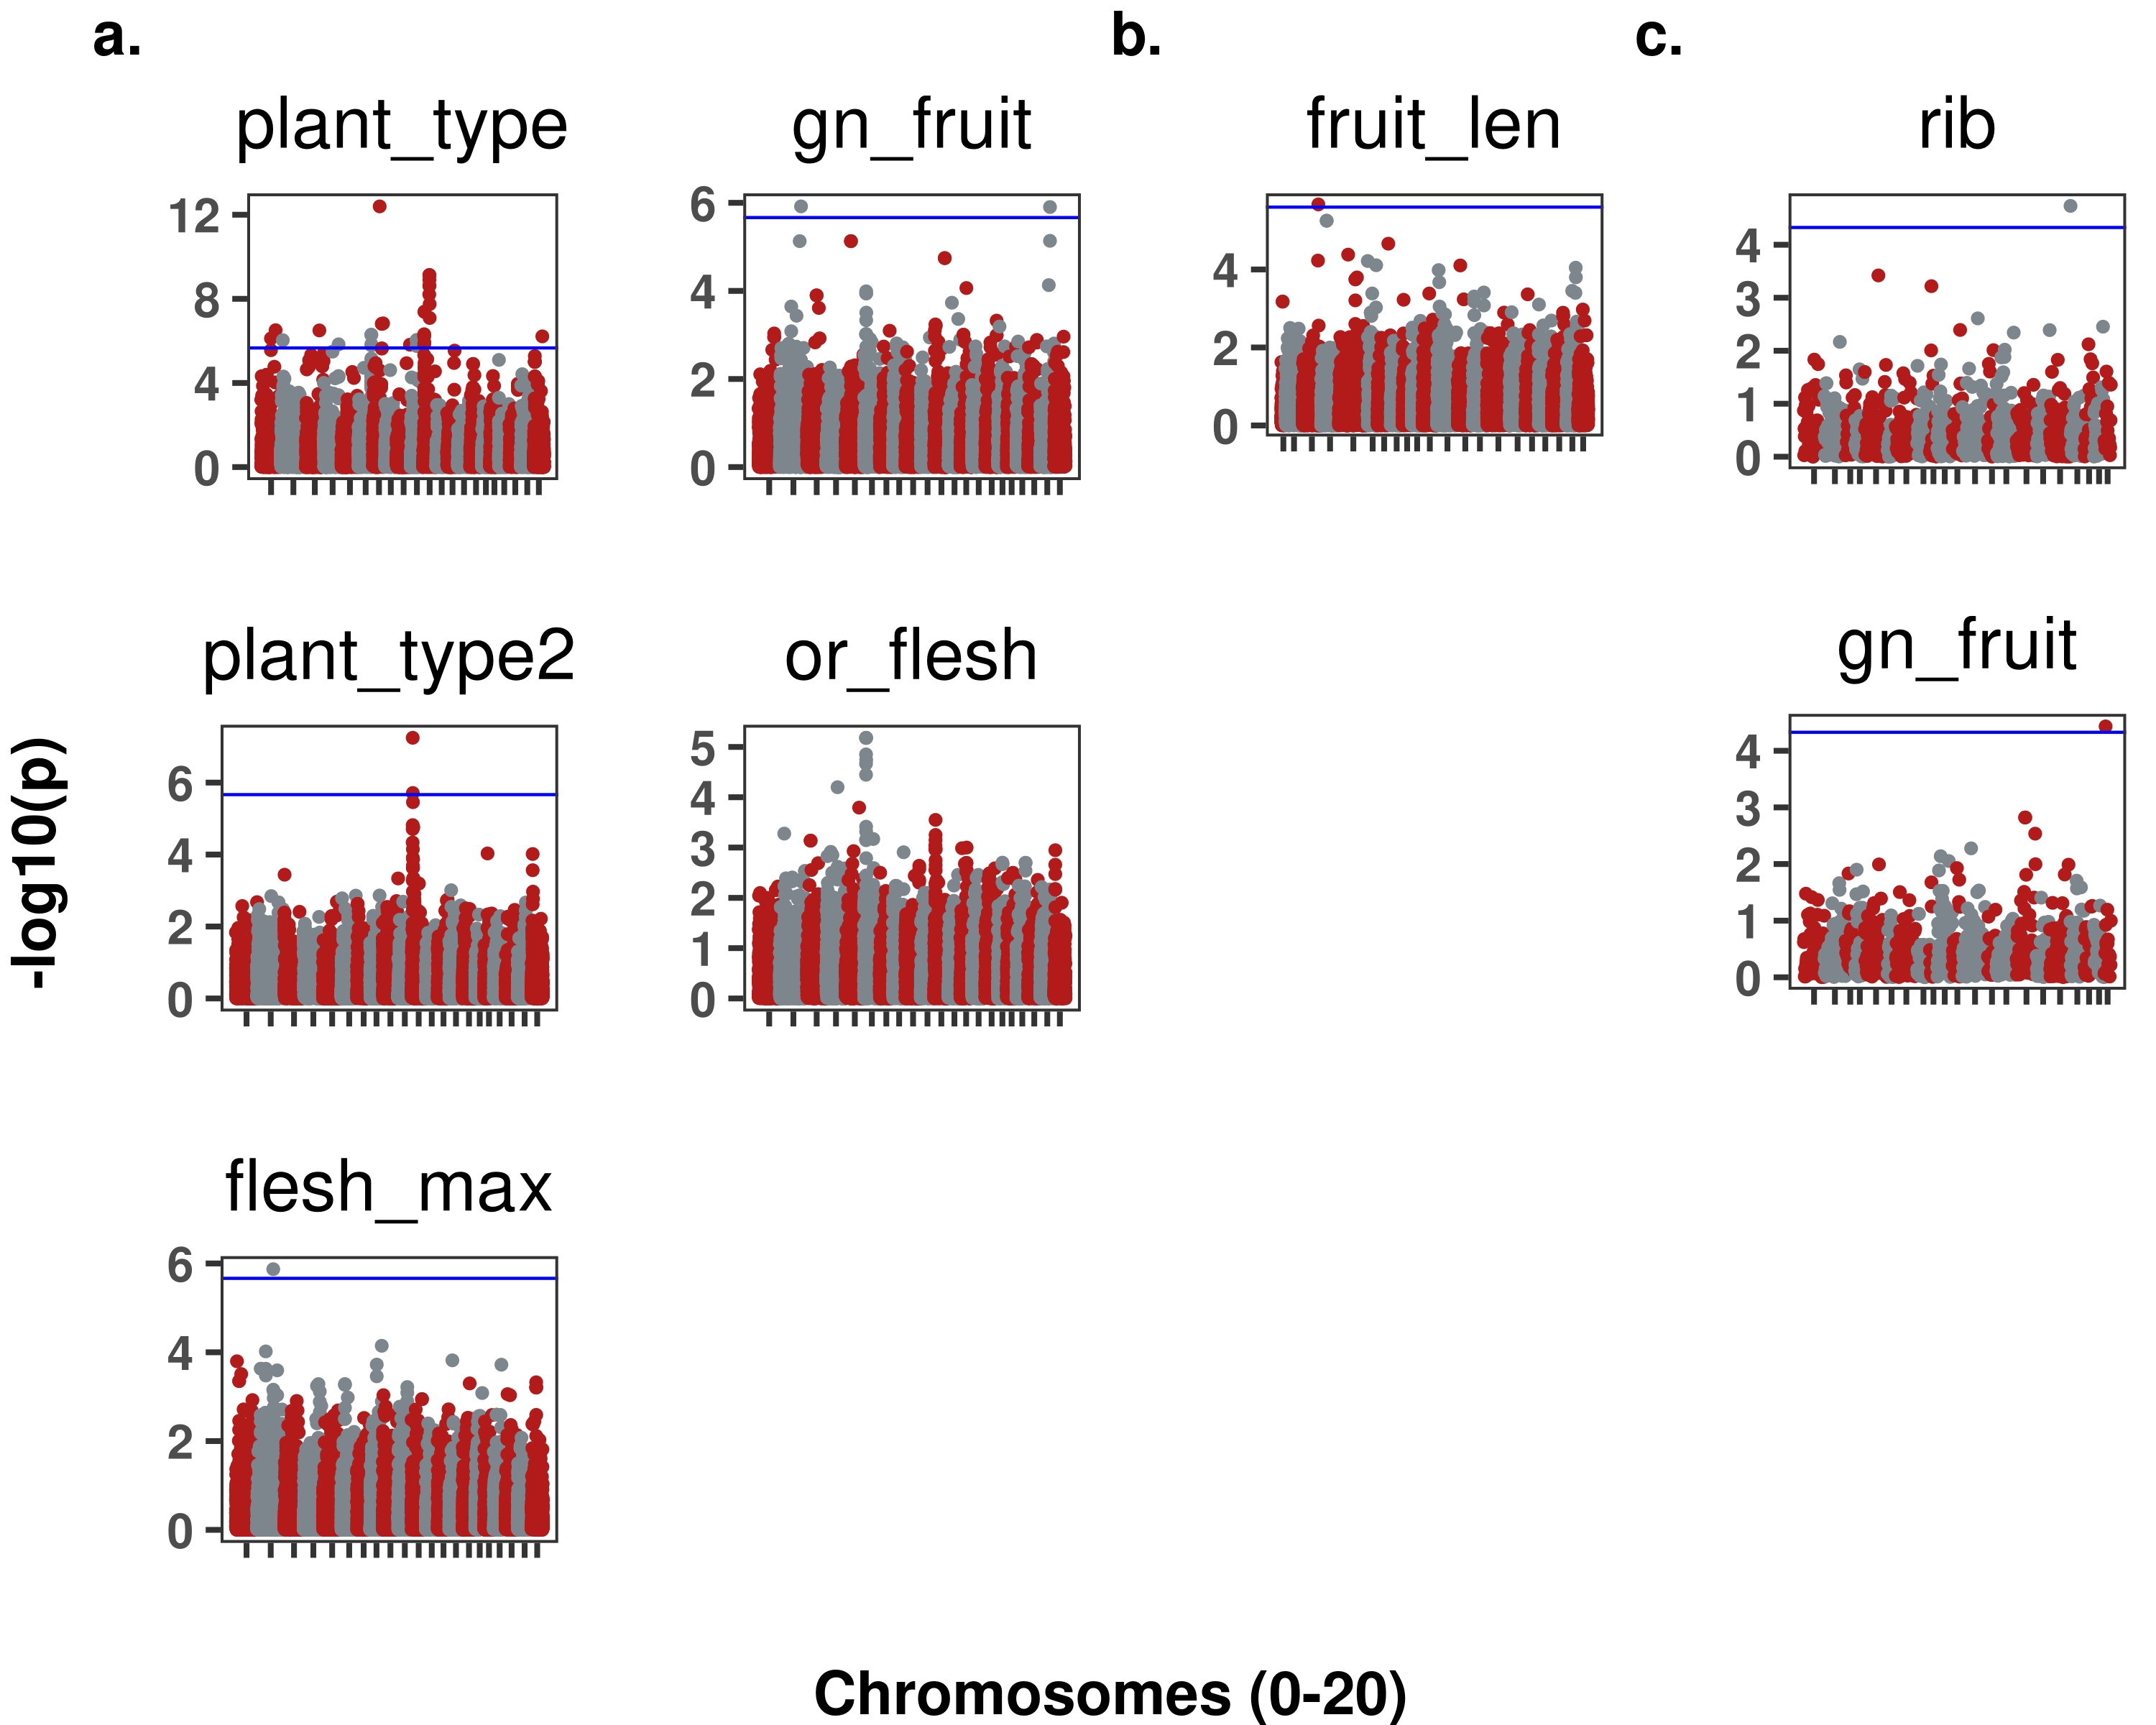
\includegraphics[width=15cm]{../../figures/04_fig.png}% This is a *.eps file
	\end{center}
	\caption{GWAS results: panel a. C. pepo plant\_type (bush or vine historical data, Bu gene), plant\_type2( bush or vine contemporary data, Bu), flesh\_max (flesh maximum thickness), gn\_fruit (green fruit color), or\_flesh (orange flesh color); panel b. C. moschata fruit\_len (fruit length); panel c. C. maxima rib (degree of fruit ribbing); gn\_fruit (green fruit color) \label{fig:4}}
\end{figure}







%%% If you don't add the figures in the LaTeX files, please upload them when submitting the article.
%%% Frontiers will add the figures at the end of the provisional pdf automatically
%%% The use of LaTeX coding to draw Diagrams/Figures/Structures should be avoided. They should be external callouts including graphics.

\newpage

\section*{Tables}

\end{document}
